\section{File Management Layer}

\begin{frame}
    \frametitle{ Components}
    \begin{figure}
        \centering
        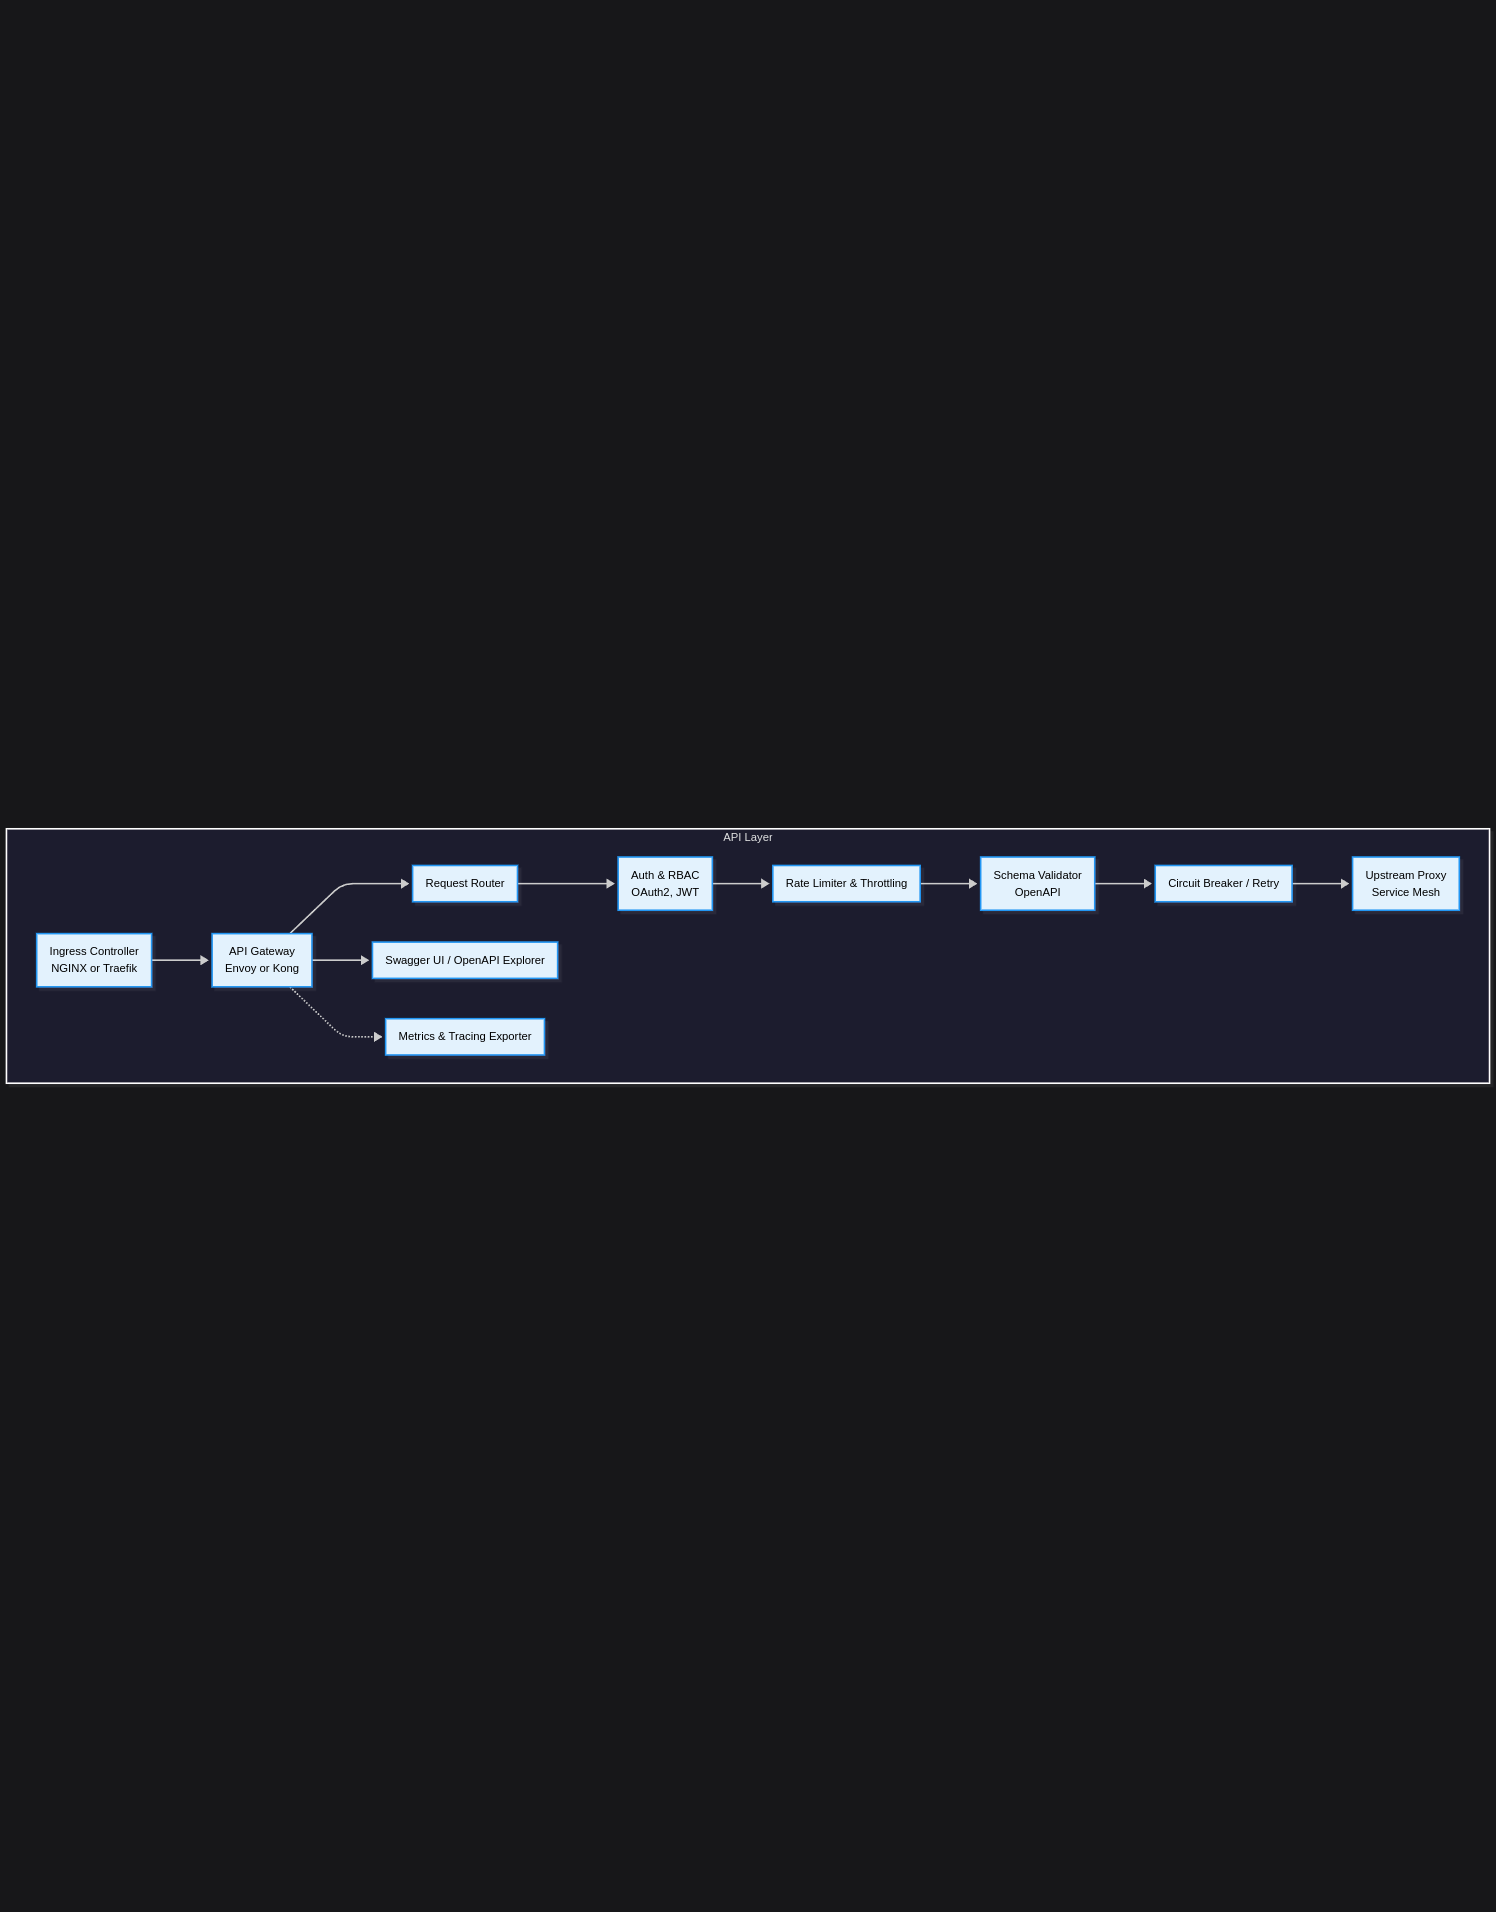
\includegraphics[width=0.8\textwidth]{file/layout.png} % Adjusted the scale of the image to 0.5
        \caption{Layout}
    \end{figure}
\end{frame}

\begin{frame}
    \frametitle{Sequence Flow}
    \begin{figure}
        \centering
        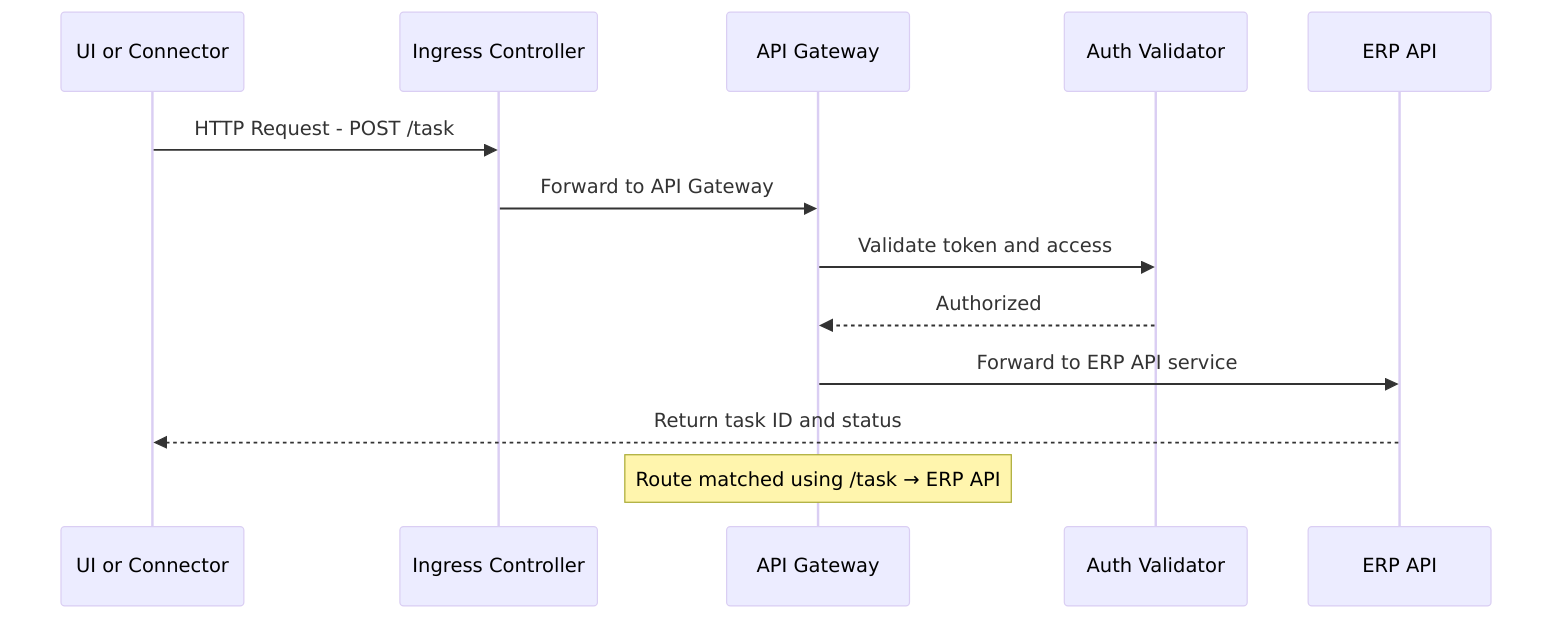
\includegraphics[width=0.8\textwidth]{file/sequence.png} % Adjusted the scale of the image to 0.5
        \caption{Sequence Flow}
    \end{figure}
\end{frame}


\begin{frame}
    \frametitle{Components}
    \begin{itemize}
        \item \textbf{File API}: Accept file uploads, fetch file versions, download final docs.
        \item \textbf{Version Controller}: Track each file's version based on hash, timestamp, origin.
        \item \textbf{Revision Detector}: Compare uploaded files with previous versions and flag differences.
        \item \textbf{Semantic Diff Engine}: Generate detailed change summaries between versions.
    \end{itemize}
\end{frame}

\begin{frame}
    \frametitle{Components}
    \begin{itemize}
        \item \textbf{Metadata Store}: Maintain file-level metadata including tags, time, uploader, task linkage.
        \item \textbf{Storage Connector}: Connect to backend storage (MinIO, S3) and perform versioned uploads.
        \item \textbf{Task Linker}: Attach or update ERP task references to versioned files.
    \end{itemize}
\end{frame}

% \begin{frame}
%     \frametitle{Technical Responsibilities - Part 1}
%     \begin{table}[h!]
% \centering
% \renewcommand{\arraystretch}{1.2}
% \begin{tabular}{|p{3cm}|p{7cm}|}
% \hline
% \textbf{Component} & \textbf{Technical Responsibility} \\
% \hline
% File API & REST endpoints or gRPC to handle uploads, downloads, and version requests \\
% \hline
% Version Controller & Uses hash (e.g., SHA-256) and timestamp to determine file lineage \\
% \hline
% Revision Detector & Triggers on new file events, compares against last version using content hash or structural diff \\
% \hline
% \end{tabular}
% \caption{File Management Layer - Technical Responsibilities (Part 1)}
% \end{table}
% \end{frame}

% \begin{frame}
%     \frametitle{Technical Responsibilities - Part 2}
%     \begin{table}[h!]
% \centering
% \renewcommand{\arraystretch}{1.2}
% \begin{tabular}{|p{3cm}|p{7cm}|}
% \hline
% \textbf{Component} & \textbf{Technical Responsibility} \\
% \hline
% Semantic Diff Engine & Uses layout-aware or LLM-based diffing on text, tables, or diagrams \\
% \hline
% Metadata Store & Backed by MongoDB or Postgres to index file metadata and history \\
% \hline
% Storage Connector & Uses MinIO or S3 SDK to store versioned blobs with immutable naming \\
% \hline
% Task Linker & Updates ERP Task Engine with version references and review status \\
% \hline
% \end{tabular}
% \caption{File Management Layer - Technical Responsibilities (Part 2)}
% \end{table}
% \end{frame}